\subsection{Experiments}

Testing the robot in a real environment presented some difficulties due to the  ultrasonic sensor limitations. The sensor has problems to detect both types of corners, convex and concave. The lack to retrieve an accurate distance on the mentioned situations impacted directly in the performance of the robot.

As seen on Figure \ref{fig:scan1}, the wall sensing is curve instead of a straight line, something not presented during simulation. This inaccuracy leads to increase the time for the particle filter to converge.
	
The time that takes to get to a random target point on the map is typically between 53-180s depending on the starting point as can be seen on Figure \ref{fig:targetReal}. 
	
		\begin{figure}[h]
			\centering
			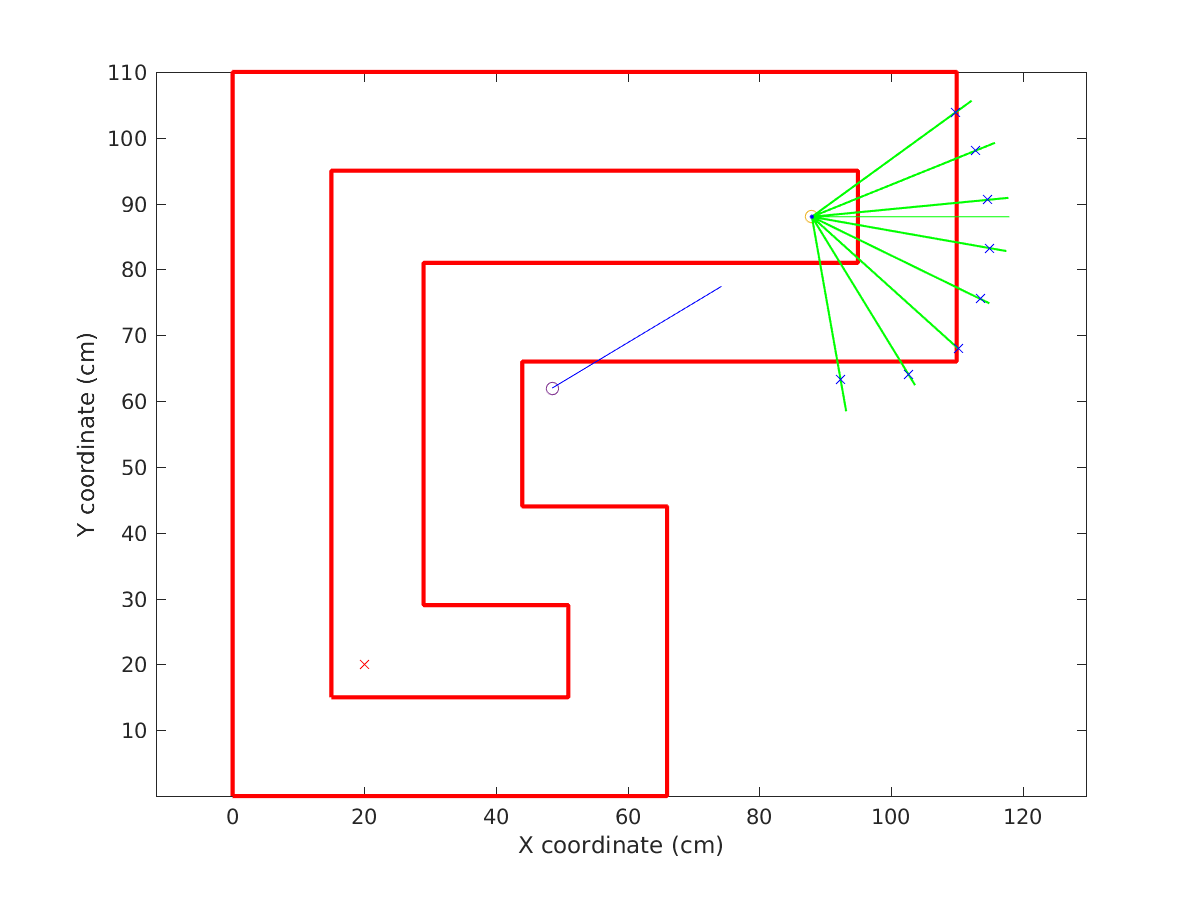
\includegraphics[scale=0.48]{scan1}
			\caption{Sensor scanning beams showing the error between the perception of the robot and the map}
			\label{fig:scan1}
		\end{figure}

		\begin{figure}[h]
			\centering
			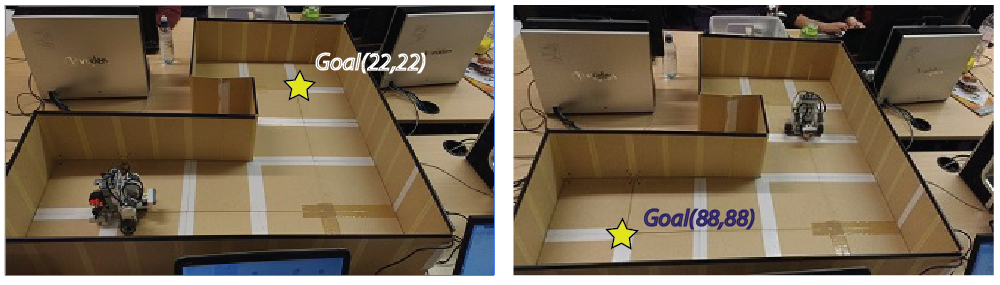
\includegraphics[scale=0.48]{targetReal}
			\caption{Sensor scanning beams showing the error between the perception of the robot and the map}
			\label{fig:targetReal}
		\end{figure}	